\documentclass[runningheads]{llncs}
\usepackage{pgfplots}
\usepgfplotslibrary{colorbrewer}
\pgfplotsset{compat=1.17}

\begin{document}

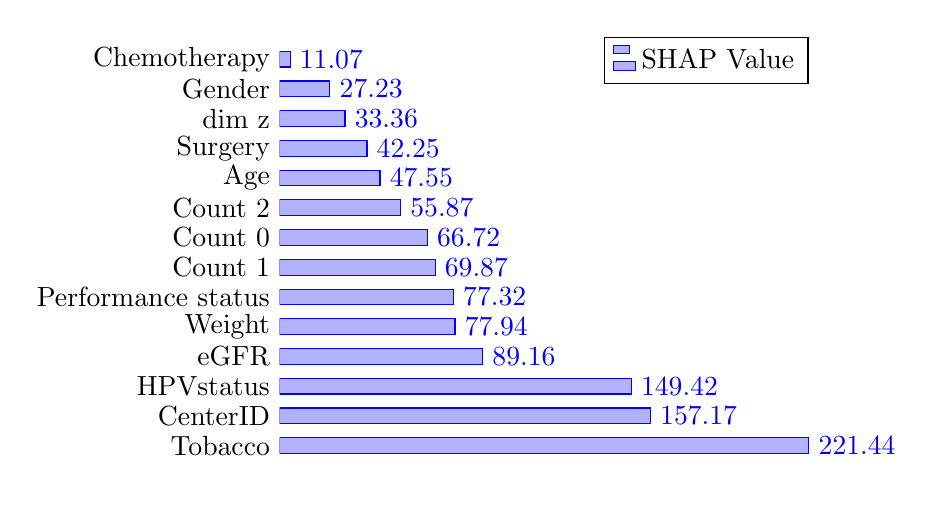
\begin{tikzpicture}
      \begin{axis}[
        xbar,
        bar width = .2cm,
        y axis line style = { opacity = 0 },
        axis x line       = none,
        tickwidth         = 0pt,
        ytick             = data,
        enlarge y limits  = 0.08,
        enlarge x limits  = 0.02,
        symbolic y coords = {
            Tobacco, CenterID, HPVstatus, eGFR, Weight, 
            Performance status, Count 1, Count 0, Count 2, Age,
            Surgery, dim z, Gender, Chemotherapy },
        nodes near coords,
      ]
      \addplot coordinates { (221.44229552224851,Tobacco) (157.16983430658996,CenterID)
                             (149.41783634574102,HPVstatus)  (89.15552515411888,eGFR)
                             (77.93642775772419,Weight)  (77.31576789744791,Performance status)
                             (69.86924467891895,Count 1)  (66.72384837570927,Count 0)
                             (55.872933522133174,Count 2)  (47.550111878156045,Age)
                             (42.24799618962943,Surgery)  (33.36418964711438,dim z)
                             (27.228049502727902,Gender)  (11.07081818789859,Chemotherapy)};
      \legend{SHAP Value}
      \end{axis}
    \end{tikzpicture}

\end{document}